% This file was created with tikzplotlib v0.10.1.
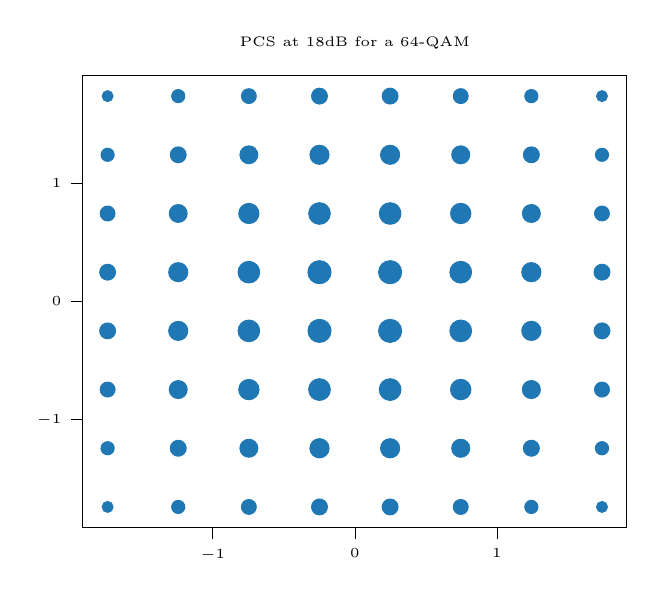
\begin{tikzpicture}[font=\tiny]

\definecolor{darkgray176}{RGB}{176,176,176}
\definecolor{steelblue31119180}{RGB}{31,119,180}

\begin{axis}[
width=0.7\columnwidth,
tick align=outside,
tick pos=left,
title={PCS at 18dB for a 64-QAM},
x grid style={darkgray176},
xmin=-1.91370995044708, xmax=1.91370995044708,
xtick style={color=black},
y grid style={darkgray176},
ymin=-1.91370995044708, ymax=1.91370995044708,
ytick style={color=black}
]
\addplot [
  draw=steelblue31119180,
  fill=steelblue31119180,
  mark=*,
  only marks,
  scatter,
  scatter/use mapped color={
	    draw=steelblue31119180,
	    fill=steelblue31119180,
	  },
  scatter/@pre marker code/.append style={/tikz/mark size=\perpointmarksize},
  visualization depends on={\thisrow{sizedata} \as\perpointmarksize}
]
table{%
x  y  sizedata
-1.73973631858826 1.73973631858826 1.9526323
-1.24266886711121 1.73973631858826 2.3550203
-0.745601296424866 1.73973631858826 2.6642342
-0.24853378534317 1.73973631858826 2.8471494
0.24853378534317 1.73973631858826 2.8471115
0.745601296424866 1.73973631858826 2.677733
1.24266886711121 1.73973631858826 2.3670127
1.73973631858826 1.73973631858826 1.9558012
-1.73973631858826 1.24266886711121 2.3550203
-1.24266886711121 1.24266886711121 2.84033
-0.745601296424866 1.24266886711121 3.213265
-0.24853378534317 1.24266886711121 3.4338744
0.24853378534317 1.24266886711121 3.4338288
0.745601296424866 1.24266886711121 3.2295456
1.24266886711121 1.24266886711121 2.8547938
1.73973631858826 1.24266886711121 2.3588421
-1.73973631858826 0.745601296424866 2.6642342
-1.24266886711121 0.745601296424866 3.213265
-0.745601296424866 0.745601296424866 3.635166
-0.24853378534317 0.745601296424866 3.8847418
0.24853378534317 0.745601296424866 3.88469
0.745601296424866 0.745601296424866 3.6535845
1.24266886711121 0.745601296424866 3.2296278
1.73973631858826 0.745601296424866 2.668558
-1.73973631858826 0.24853378534317 2.8471494
-1.24266886711121 0.24853378534317 3.4338744
-0.745601296424866 0.24853378534317 3.8847418
-0.24853378534317 0.24853378534317 4.151452
0.24853378534317 0.24853378534317 4.1513968
0.745601296424866 0.24853378534317 3.9044247
1.24266886711121 0.24853378534317 3.451361
1.73973631858826 0.24853378534317 2.85177
-1.73973631858826 -0.24853378534317 2.8471115
-1.24266886711121 -0.24853378534317 3.4338288
-0.745601296424866 -0.24853378534317 3.88469
-0.24853378534317 -0.24853378534317 4.1513968
0.24853378534317 -0.24853378534317 4.1513414
0.745601296424866 -0.24853378534317 3.904373
1.24266886711121 -0.24853378534317 3.451315
1.73973631858826 -0.24853378534317 2.8517323
-1.73973631858826 -0.745601296424866 2.677733
-1.24266886711121 -0.745601296424866 3.2295456
-0.745601296424866 -0.745601296424866 3.6535845
-0.24853378534317 -0.745601296424866 3.9044247
0.24853378534317 -0.745601296424866 3.904373
0.745601296424866 -0.745601296424866 3.6720963
1.24266886711121 -0.745601296424866 3.2459917
1.73973631858826 -0.745601296424866 2.6820786
-1.73973631858826 -1.24266886711121 2.3670127
-1.24266886711121 -1.24266886711121 2.8547938
-0.745601296424866 -1.24266886711121 3.2296278
-0.24853378534317 -1.24266886711121 3.451361
0.24853378534317 -1.24266886711121 3.451315
0.745601296424866 -1.24266886711121 3.2459917
1.24266886711121 -1.24266886711121 2.8693318
1.73973631858826 -1.24266886711121 2.3708544
-1.73973631858826 -1.73973631858826 1.9558012
-1.24266886711121 -1.73973631858826 2.3588421
-0.745601296424866 -1.73973631858826 2.668558
-0.24853378534317 -1.73973631858826 2.85177
0.24853378534317 -1.73973631858826 2.8517323
0.745601296424866 -1.73973631858826 2.6820786
1.24266886711121 -1.73973631858826 2.3708544
1.73973631858826 -1.73973631858826 1.9589754
};
\end{axis}

\end{tikzpicture}
